\documentclass[a4paper,12pt]{extarticle}
\usepackage[margin=1.5cm]{geometry}
\usepackage{amsmath, amssymb}
\usepackage{array}
\usepackage{multicol}
\usepackage{helvet}
\usepackage{multirow}
\usepackage{graphicx}
\renewcommand{\baselinestretch}{2}
\renewcommand{\familydefault}{\sfdefault}

\begin{document}

    \begin{tabular}{| c | c | c | c |}
        \hline
        & MATEMÁTICAS & 25/03/2026 & calificación \\
        \hline 

        \multirow{2}{*}{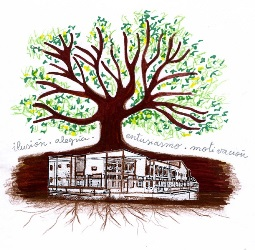
\includegraphics{../../img-Logos/iesoGalileo.jpg}} & Nombre y apellidos \hspace{120pt} & Ex. 2º ESO   & \\ 
        &&Rec. 1ºESO (parte2 )& \\ 
        \hline
    \end{tabular}
    
    \begin{tabular}{| l | }
        \hline
        NOTAS: \\ 
            1. El examen tiene que ser limpio, ordenado y sin faltas de ortografía. \\
            
            2. El examen ha de realizarse en bolígrafo negro o azul, evitando tachones en la medida \\
            de lo posible. \\ 
            
            3. Deben aparecer todas las operaciones NO vale con indicar solo el resultado.\\
            
            4. Los problemas deben contener: Datos, planteamiento y resolución, respondiendo a lo \\
            que se pregunte, NO vale con indicar un número como solución del problema.\\

            5. Persona que se vea copiando o hablando con un compañero tiene un cero en el examen\\

            6. NO está permitido el uso de calculadoras \\
        \hline
    \end{tabular}

    \begin{enumerate}
        \item Dados los polinomios 
            \[P(x) = 2x^5+3x-2  \qquad \qquad Q(x) = 3x^5+x^2-7x+1\]
            Calcula: \\
                (a) P(x)+Q(x) $ \qquad \qquad  \qquad  \qquad  \qquad  \qquad  \qquad  \qquad  $ (b) Q(x)-P(x)
            $\vspace{3cm}$ 
        
        \item Resuelve las siguientes ecuaciones:
        
            (a)$8x-5x=x+8 \qquad  \qquad  \qquad  \qquad  \qquad $ 
            (b) $2x-8=1-3(x-2)$ $\vspace{4cm}$ 
        \item Completa la tabla para cada uno de los monomios siguientes.
        
            \begin{tabular}{| c | c | c | c |}
                \hline
                Monomio & Coeficiente & Parte literal & Grado \\
                \hline
                $2a$&&&\\ 
                \hline
                $x^2$&&&\\ 
                \hline
                $-3ab$&&&\\ 
                \hline
                $\dfrac{1}{2}xy^3$&&&\\ 
                \hline
            \end{tabular}

        \item 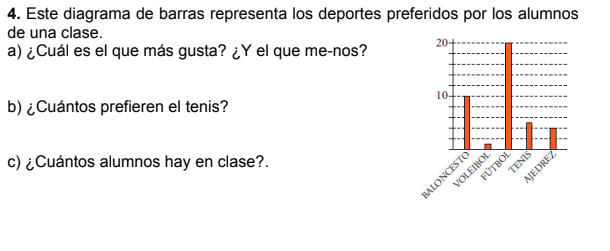
\includegraphics{img/pregunta4,estadistica.png}$\vspace{2cm}$ 
        \item Si al doble de un número se le resta su mitad, resulta 54. Hallar ese número. $\vspace{4cm}$ 
        \item Seis obreros descargan un camión en tres horas. ¿Cuánto tardarán cuatro obreros? $\vspace{4cm}$ 
        \item 200 g de jamón cuestan 4 €. ¿Cuánto costarán 150 gramos? $\vspace{4cm}$ 
        \item Calcula:\\
                (a) 50\% de 620 \\
                (b) 7\% de 444 
                $\vspace{4cm}$ 

        \item Las notas del último examen de matemáticas de seis amigos son:

                        9, 5, 10, 5, 7, 6

                    Halla la media, la mediana, la moda y el recorrido de las notas.$\vspace{4cm}$ 
        \item En el experimento aleatorio consistente en lanzar un dado,
        \begin{enumerate}
            \item ¿Qué probabilidad hay de obtener un múltiplo de 2?
            \item Halla la probabilidad de sacar número primo.
            \item ¿Qué probabilidad hay de sacar un número impar?
        \end{enumerate}
    \end{enumerate}
\end{document}